\documentclass[a4paper,12pt]{article}
\usepackage{graphicx}
\usepackage{enumitem} 
\usepackage{hyperref} 
\usepackage{listings}


\hypersetup{
    colorlinks=true,
    linkcolor=blue,
    filecolor=magenta,      
    urlcolor=cyan,
    pdftitle={Overleaf Example},
    pdfpagemode=FullScreen,
    }


    
\usepackage{xcolor}
\usepackage[a4paper, top=0.8in, bottom=0.8in, left=0.8in, right=0.8in]{geometry}
\usepackage{array}
\usepackage{tabularx}
\usepackage{multirow}
\usepackage{url}

\title{\textbf{PTC Quality Control Test Setup \\ \& Quality Control Procedure}}
\author{}
\date{}

\begin{document}

\maketitle


\begin{center}
\renewcommand{\arraystretch}{1.2}  % More vertical spacing
\begin{tabularx}{\textwidth}{|l|l|l|X|}
\hline
\textbf{Version} & \textbf{Date} & \textbf{Author} & \textbf{Notes} \\
\hline
v0.0 & 2025-11-21 & A. Nikolica & Initial draft \\
v0.1 & 2025-12-03 & D. Drobner & Add JTAG in-situ programming \\
v1.0 & 2025-12-03 & A. Nikolica & Add WEIC figure in last section \\
v1.1 & 2026-03-26 & A. Nikolica & Corrections in dune-daq section \\
\hline

\end{tabularx}
\end{center}

\vspace{2em}  


\tableofcontents
\newpage

\section{Introduction}

This document will guide the reader through the process of testing the Power and Timing Cards (PTCs) used in the DUNE experiment. PTCs sit outside the cryostat and operate at ambient temperature. There is one PTC per warm electronics interface crate (WEIC) which powers up to 6 warm interface boards (WIBs) in the WEIC with 12V at up to 6A. Each DC-DC converter to a WIB can be turned on an off independently. The PTC fans out the encoded timing stream from its front panel SFP to each WIB, and accepts timing transmission back from one WIB at a time via a priority encoding scheme. PTC can monitor its own voltages, currents, and some PCB surface temperatures. It also has an I2C interface to WIBs for sensor reading or arbitrary communication with the FPGA. The PTC has an EtherCAT interface to the detector safety system (DSS), and a gigabit Ethernet (GbE) interface to the slow control (SC) system.  

\vskip 1 cm

The procedure includes three main stages: 

\begin{itemize}
    \item Reception check: photo taking, visual inspection, vendor documentation check
    \item QC testing: determine that components are installed correctly by running functional tests for power up, and FPGA and microcontroller programming
    \item Installation of front panels and heatsinks, and storage for shipping
\end{itemize}

\vskip 1 cm

The document is structured as follows:

\begin{itemize}
    \item Section~\ref{section:equipment} provides a detailed overview of all equipment used during QC testing: hardware, software, and tools
    
    \item Section~\ref{section:overview} offers a quick view of the workflow of each of the processes in the QC testing
    
    \item Section~\ref{section:procedure} shows the step by step procedures required to perform the QC tests
    
\end{itemize}



\vskip 1cm

\textbf{We strongly recommend that the reader goes through this manual entirely before starting to perform any tests}.
%%%%%%%%%%%%%%%%%%%%%%%%%%%%%%%%%%%%%%%%%%%%%%%%%%%%%%%


%%%%%%%%%%%%%%%%%%%%%%%%%%%%%%%%%%%%%%%%%%%%%%%%%%%%%%%

\clearpage

\section{List of Equipment}
\label{section:equipment}

Tables~\ref{tab:visual_components}-\ref{tab:tester_wearing} describe all the equipment necessary to perform the QC tests. 

\subsection{Visual Inspection}

\begin{table}[h]
    \centering
    \renewcommand{\arraystretch}{1.3} 
    \begin{tabularx}{\textwidth}{|c|X|X|}
        \hline
        \textbf{Code} & \textbf{Name} & \textbf{Notes} \\ 
        \hline
        101 & Digital camera capable of 12MP &  For taking high resolution photographs of both sides of assembled boards \\ 
        \hline
        102 & Microscope and camera &  For reception checkout of defects in front panels and bare PCBs \\ 
        \hline
        103 & Code Scanner & \href{https://tera-digital.com/products/d6100-2d-wireless-barcode-scanner-with-stand}{Tera 1D \& 2D Scanner} with base and bluetooth dongle, for entering assembled PCBs into DUNE HWDB  \\
        \hline
    \end{tabularx}
    \caption{List of visual inspection components and their corresponding codes}
    \label{tab:visual_components}
\end{table}

\vskip 1 cm

    \begin{figure}[h!]
        \centering
        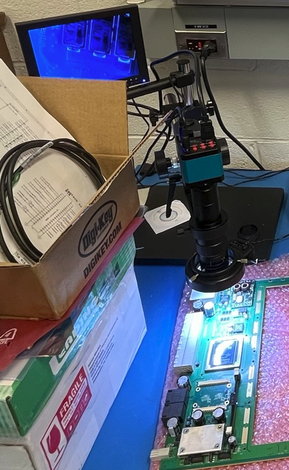
\includegraphics[scale=1.25]{images/microscope.png} 
        \caption{Visual inspection components (microscope and camera)}
        \label{microscope}
    \end{figure}

    \begin{figure}[h!]
        \centering
        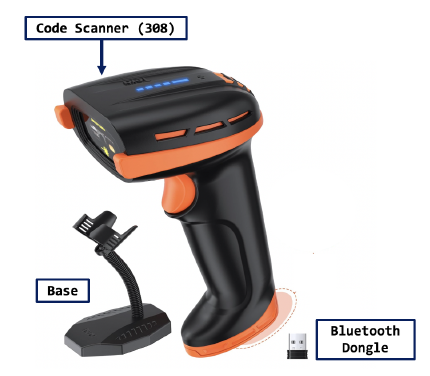
\includegraphics[scale=1]{images/scanner.png} 
        \caption{Visual inspection components (scanner)}
        \label{scanner}
    \end{figure}

\newpage
\subsection{QC Board Test Station}
The QC board is the main test structure which PTC plugs into. All the associated hardware and software are listed in Table~\ref{tab:qc_components}, and illustrated in Figures~\ref{qc_test_stand} -- Figures~\ref{qc_test_stand_close}.

\begin{table}[h]
    \centering
    \renewcommand{\arraystretch}{1.1} 
    \begin{tabularx}{\textwidth}{|c|X|X|}
        \hline
        \textbf{Code} & \textbf{Name} & \textbf{Notes} \\ 
        \hline
        201 & QC test board &  Main test structure, with strain relief structure for cabling \\ 
        \hline
        202 & 24V @ 3A laboratory power supply and cable  &  24V for QC board, 12V for cooling fans \\ 
        \hline
        203 & 48V @ 12.5A power supply  &  For PTC device under test (DUT) \\ 
        \hline
        204 & Oscilloscope, at least 2 channels and probes, at least 100MHz bandwidth  &  For probing QC board test points (and PTC test points if required for debugging) \\ 
        \hline
        205 & Digital volt meter (DVM)  &  For probing test points\\ 
        \hline
        206 & Linux machine  &  For test scripts, timing server, HWDB \\ 
        \hline
        207 & 3x Ethernet cables  &  For QC board, PTC GbE connection, and EtherCAT connection \\ 
        \hline
        208 & GbE media converter & 10GTek A7S2-33-1GX1GT-SFP/GT3 for PTC front panel to network switch \\ 
        \hline
        209 & GbE network switch & For connecting PTC and QC board to Linux machine  \\ 
        \hline
        210 & Windows machine  & For running Beckhoff TwinCAT (EtherCAT software) \\ 
        \hline
        211 & 10/100 media converter &  tp-link MC100CM Fast Ethernet Media Converter, for connecting PTC front panel to Windows machine \\ 
        \hline
        212 & 3x SFP modules & 10Gtek ASF85-24-X2-D (GbE), SFP-100FX-31-I, FS P/N 12713 (EtherCAT), SFP1G-SX-85, FS P/N 11774 (timing) \\ 
        \hline
        213 & 3x fibers & 1m LC to LC OM1, FS P/N 42095 (GbE and timing), 1m LC to SC OM3, FS P/N 41751 (EtherCAT) \\
        \hline
        214 & SD card writer & For preparing bootable SD cards for PTC \\
        \hline
        215 & Microcontroller programming pod & Infineon XMD Link, for XMC-4300 \\
        \hline
    \end{tabularx}
    \caption{List of QC test stand components and their corresponding codes}
    \label{tab:qc_components}
\end{table}

\vskip 0.8 cm

    \begin{figure}[h!]
        \centering
        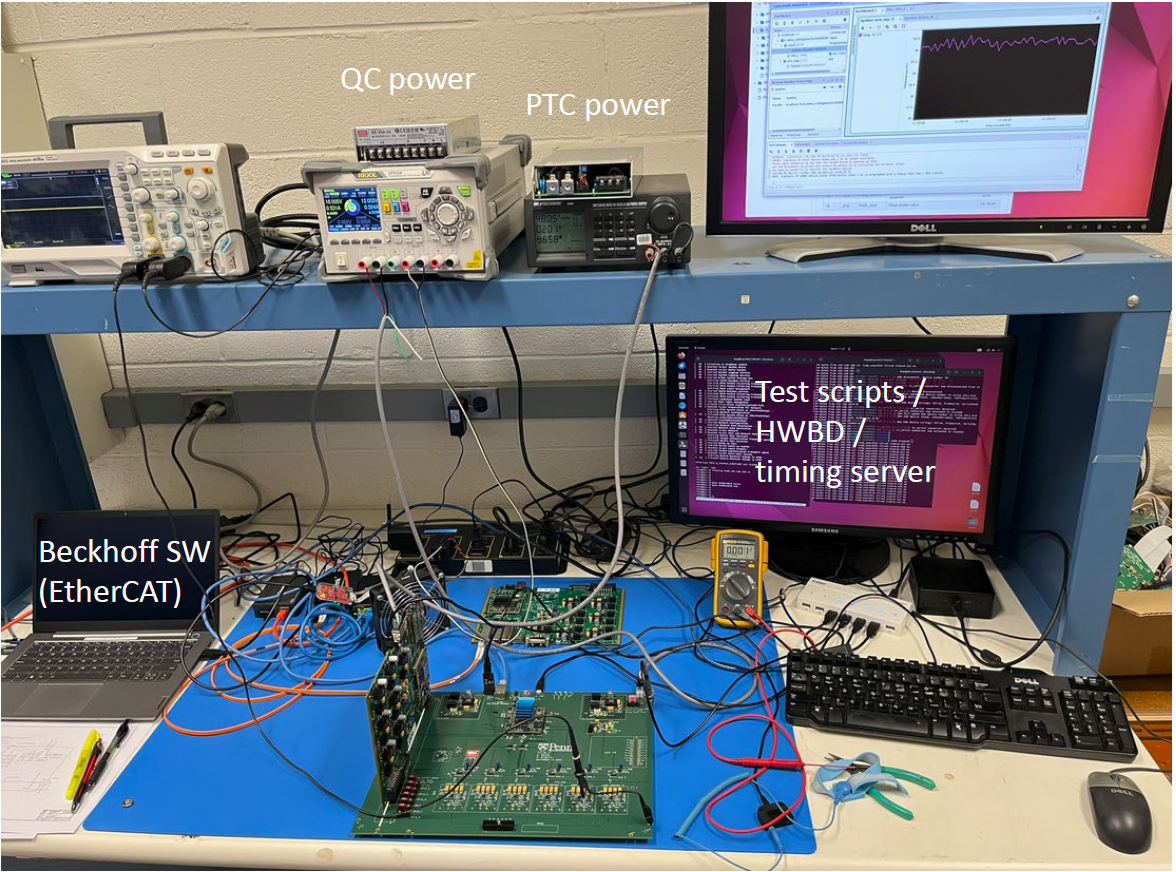
\includegraphics[scale=0.7]{images/qc_test_stand.png} 
        \caption{PTC test setup}
        \label{qc_test_stand}
    \end{figure}

\newpage

\vskip 0.8 cm

    \begin{figure}[h!]
        \centering
        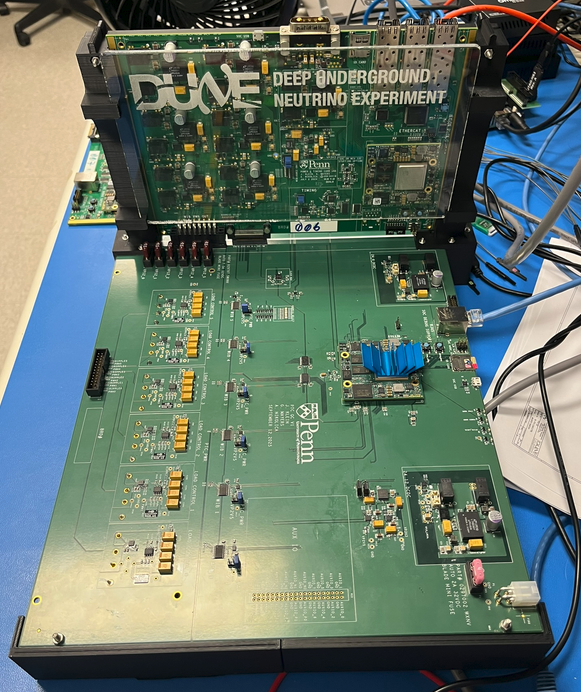
\includegraphics[scale=1.0]{images/qc_test_stand_close.png} 
        \caption{Closeup of QC board and DUT}
        \label{qc_test_stand_close}
    \end{figure}


\newpage
\subsection{Personal Protective Equipment (PPE) for Tester}

The list of PPE that the tester should wear while performing QC tests is shown in Table~\ref{tab:tester_wearing}, and illustrated in Figure~\ref{PPE_parts}.

\begin{table}[h]
    \centering
    \renewcommand{\arraystretch}{1.3} 
    \begin{tabularx}{\textwidth}{|c|X|X|}
        \hline
        \textbf{Code} & \textbf{Name} & \textbf{Notes} \\ 
        \hline
        301 & Long Pants &  \\ 
        \hline
        302 & Long Sleeve Top &   \\ 
        \hline
        303 & Closed Toe Shoes &    \\ 
        \hline
        304 & ESD-safe gloves or Latex gloves  & While plugging/unplugging newly assembled PTCs into QC board \\ 
        \hline
        305 & Antistatic Wrist Strap  & Connect to ESD monitoring while handling hardware   \\ 
        \hline
    \end{tabularx}
    \caption{List of PPE for the tester to wear during QC tests.}
    \label{tab:tester_wearing}
\end{table}

    \begin{figure}[h!]
        \centering
        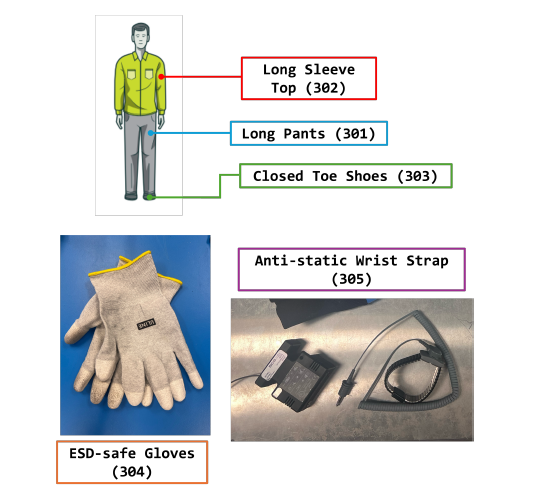
\includegraphics[scale=1.0]{images/ppe_parts.png} 
        \caption{PPE Components}
        \label{PPE_parts}
    \end{figure}


%%%%%%%%%%%%%%%%%%%%%%%%%%%%%%%%%%%%%%%%%%%%%%%%%%%%%%%%%%%%%%%%%%%%%%%%%%%%%%%%%%
\newpage

\section{Quick Overview of the Operation Procedure}
\label{section:overview}

The overall operation procedure consists of 4 phases: reception checks, manual QC tests, semi-automated QC tests, and final assembly. The reception checks consist of examining front panels and bare PCBs before components are assembled onto the PTCs. After the components are installed and delivered from the assembler, photos are taken and polarized component orientations are checked. A high level overview of these steps are in EDMS document 338406. Manual QC tests consist of measurements that must be taken with DVM or oscilloscope, and tests that involve asserting DIP switches or jumpers on the boards. Semi-automated tests are run by script and generate text output. Final assembly involved installing heatsinks and front panels, and preparing the boards for packaging and shipment.

%%%%%%%%%%%%%%%%%%%%%%%%%%%%%%%%%%%%%%%%%%%%%%%%%%%%%%%
\newpage


\section{Itemized QC Procedure}
\label{section:procedure}

\subsection{Reception Checkout}
\label{section:reception_checkout}

    \textbf{Note:} For all visual inspections, the \textcolor{blue}{\textbf{Acceptance criteria: PASS/FAIL}}.

\subsubsection{Visual Inspection of Front Panels}
\label{section:visual_inspection}

An example front panel is shown in Figure~\ref{front_panel}. The orders of front panels should be examined as follows:

    \begin{enumerate}
        \item \textbf{Identification and Counting} – Verify that the correct number of panels has been received as per the purchase order.
        \item \textbf{Visual Inspection} – A sample (10\%) of panels should be examined under the microscope for cleanliness and any signs of physical damage, scratches, or any other defects that could impact functionality. Verify that all required components (e.g., thumb screws) are included.
        \item \textbf{Mechanical fit check} – A sample (10\%) of panels should be used to verify overall dimensions, as well as the positions and sizes of mounting holes and connector openings, against the official drawings.
    \end{enumerate}

The front panels are not tracked in the DUNE HWDB and not serialized. Any non-conforming panels shall be segregated into a separate box labeled "Rejected front panels" and reported to a UPenn electronics engineer. The non-conformance issues will be reported to the vendor.

    \begin{figure}[h!]
        \centering             
        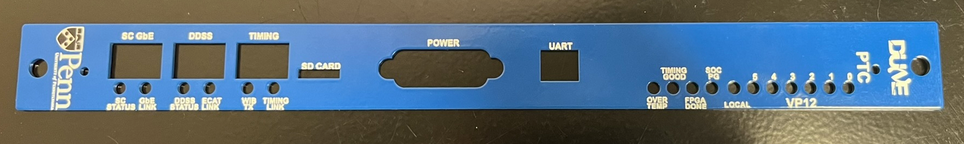
\includegraphics[scale=0.8]{images/front_panel.png}
            \caption{Example PTC front panel}
        \label{front_panel}
    \end{figure}

\subsubsection{Visual Inspection of Bare PCBs}
\label{section:visual_inspection2}

An example bare PCB is shown in Figure~\ref{bare_pcb}. The PCBs will arrive from the vendor packaged in ESD safe bags. Do not open the bags for the production PCBs. Sample boards will arrive separately packaged. These samples boards should be removed from their plastic bags to be examined.

    \begin{enumerate}
        \item \textbf{Identification and Counting} – Verify that the correct number of PCBs has been received as per the purchase order.
        \item \textbf{Reviewing quality certificates}
            \begin{enumerate}
                \item Examine the Quality Certificate and QC test reports provided by the vendor and fill the designated form on \href{https://docs.google.com/spreadsheets/d/10I7u4FrWQXx4R3NOPhapa5DsjlLhDk9keJTLW0Wgq5A/edit?gid=0#gid=0}{GoogleDoc}. Document any issues in the “Notes” section in the form. If any problems are identified, notify the QC representative.
                \item Download the completed form from GoogleDoc as Spreadsheet in Microsoft Excel and PDF formats and upload both files to DUNE HWDB.
                \item Make a copy of QC certificates and test reports and upload them to DUNE HWDB. 
            \end{enumerate}
        \item \textbf{Visual Inspection of Sample PCBs}
            \begin{enumerate}
                \item Inspect the Sample Boards under the microscope according to the check list provided on \href{https://docs.google.com/spreadsheets/d/10I7u4FrWQXx4R3NOPhapa5DsjlLhDk9keJTLW0Wgq5A/edit?gid=0#gid=0}{GoogleDoc} and fill the form. Use the provided reference PCB to make a judgment on various check items. Record any problems in the “Notes” section in the form. If defects are found, notify the QC representative. The checklist is reproduced here for clarity:
                \begin{enumerate}
                        \item Overall PCB appearance and cleanliness 
                        \item Surface quality: existence of pit, scratch or pin holes on printing traces or pad
                        \item Inspect PCB edges for possible defects
                        \item Inspect both sides of PCB
                        \item Check for any other noticeable defects, damages, irregularities, etc.
                    \end{enumerate}
                \item Download the completed form from GoogleDoc as Spreadsheet in Microsoft Excel and PDF formats and upload both files to DUNE HWDB.
                \item Attach a sticker to the Sample Board with the following information: 
                    \begin{enumerate}
                        \item PCB serial number 
                        \item PCB production batch number
                        \item Inspection date
                        \item Initials and last name of the person who performed the inspection
                    \end{enumerate}
            \end{enumerate}            
    \end{enumerate}

The PTCs are not tracked by serial number until the assembly process is complete. Any non-conforming sample bare PCBs at this stage shall be segregated into a separate box labeled "Rejected bare PCBs" and reported to a UPenn electronics engineer. The non-conformance issues will be reported to the vendor.

    \begin{figure}[h!]
        \centering             
        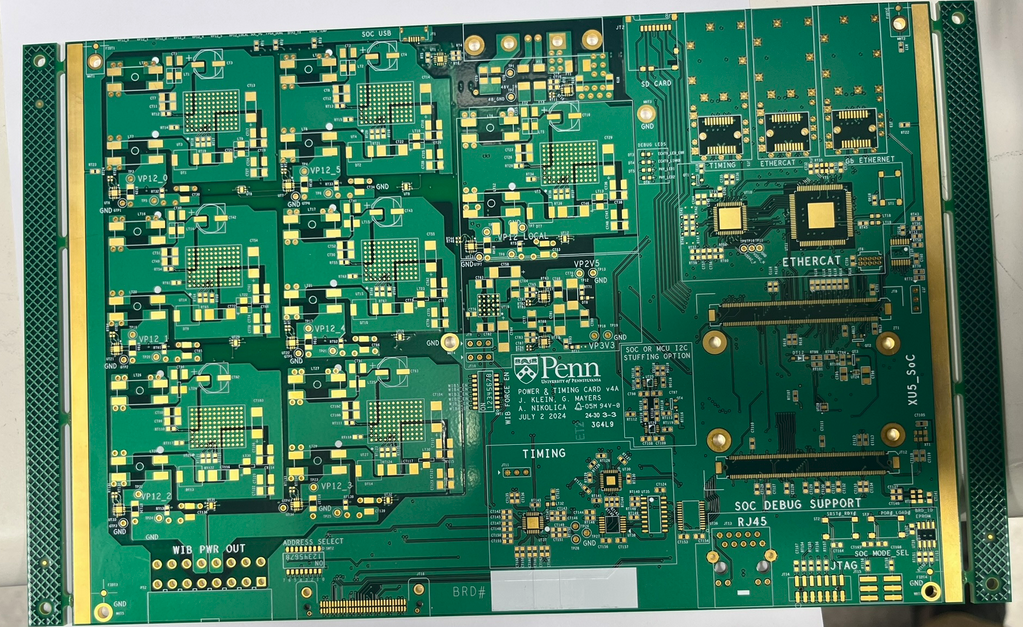
\includegraphics[scale=0.8]{images/bare_pcb.png}
            \caption{Example bare PCB}
        \label{bare_pcb}
    \end{figure}

\subsubsection{Visual Inspection of Assembled PCBs}
\label{section:visual_inspection3}

An example of an assembled PCB is shown in Figure~\ref{assembled_pcb}. The PCBs will arrive from the vendor packaged in ESD safe bags. At this stage, all PPE should be worn to prevent damage from ESD discharge and contamination.

    \begin{enumerate}
        \item \textbf{Identification and Counting} – Verify that the correct number of PCBs has been received as per the purchase order.
        \item \textbf{Reviewing quality certificates}
            \begin{enumerate}
                \item Examine the Quality Certificate and QC test reports provided by the vendor and fill the designated form on \href{https://docs.google.com/spreadsheets/d/10I7u4FrWQXx4R3NOPhapa5DsjlLhDk9keJTLW0Wgq5A/edit?gid=0#gid=0}{GoogleDoc}. Document any issues in the “Notes” section in the form. If any problems are identified, notify the QC representative.
                \item Download the completed form from GoogleDoc as Spreadsheet in Microsoft Excel and PDF formats and upload both files to DUNE HWDB.
                \item Make a copy of QC certificates and test reports and upload them to DUNE HWDB. 
            \end{enumerate}
        \item \textbf{Visual Inspection of Sample PCBs}
            \begin{enumerate}
                \item Take a high resolution photograph of the front and back of the boards, and upload to the DUNE HWDB.
                \item Inspect each assembled PCB under the microscope according to the check list provided on \href{https://docs.google.com/spreadsheets/d/10I7u4FrWQXx4R3NOPhapa5DsjlLhDk9keJTLW0Wgq5A/edit?gid=0#gid=0}{GoogleDoc} and fill the form. Use the provided reference PCB to make a judgment on various check items. Record any problems in the “Notes” section in the form. If defects are found, notify the QC representative. The checklist is reporduced here for clarity:
                  \begin{enumerate}
                        \item Missing solder joints, particularly on through-hole components that also have surface-mount (SMD) pins
                        \item Excess solder paste or bridging between adjacent pins
                        \item Unintended components left on the board (e.g., from pick-and-place errors)
                        \item Residues or contamination due to insufficient cleaning during assembly
                        \item Missing components (DDR memory, jumpers, etc.)
                        \item Incorrect orientation of ICs and polarized components (check pin 1 marker on ICs, and [+] marker on tantalum and polymer capacitors)
                    \end{enumerate}
                \item Document any observed issues and include a written description of the defect as well as a closeup photograph of the defect.
                \item Tag any non-conforming boards as "Visual Inspection Failed" and segregate them into a box labeled "Rejected Assembled PCBs".
                \item All boards, whether pass or fail, will have their serial codes scanned into the DUNE HWDB, and the result of the pass or fail will be noted.
                \item Download the completed form from GoogleDoc as Spreadsheet in Microsoft Excel and PDF formats and upload both files to DUNE HWDB.
            \end{enumerate}            
    \end{enumerate}

Any bare PCBs rejected from the visual inspection process and placed in the box labeled "Rejected bare PCBs" shall be reported to a UPenn electronics engineer. The non-conformance issues will be reported to the vendor.

    \begin{figure}[h!]
        \centering             
        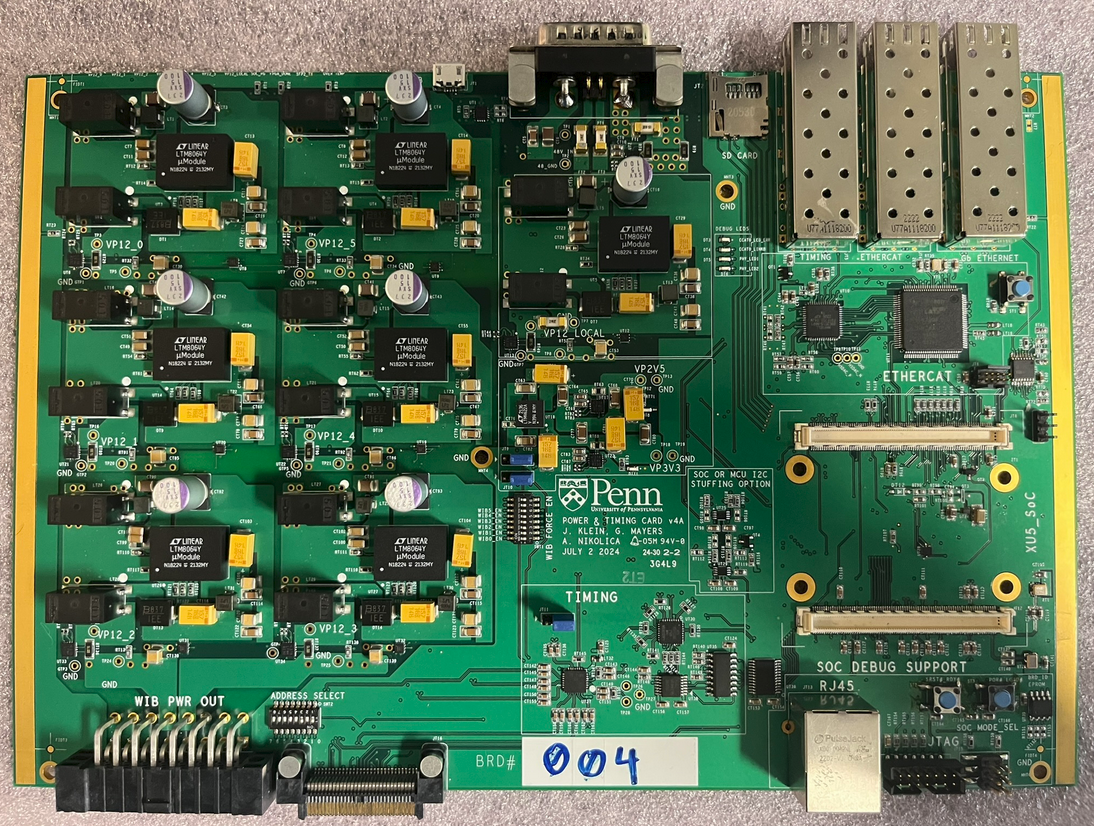
\includegraphics[scale=0.75]{images/assembled_pcb.png}
            \caption{Example assembled PCB}
        \label{assembled_pcb}
    \end{figure}


%%%%%%%%%%%%%%%%%%%%%%%%%%%%%%%%%%%%%%%%%%%%%%%%%%%%%%%
\newpage
\subsection{QC Test Stand Preparation}
\label{section:qc_prep}

\subsubsection{\texttt{dune-daq} Setup}
\label{section:dune_daq}

    The software needed for \texttt{dune-daq} is \href{https://dune-daq-sw.readthedocs.io/en/latest/}{here}. Refer to the installation guide \href{https://dune-daq-sw.readthedocs.io/en/latest/packages/daq-buildtools/}{here}.

    \begin{enumerate}
        \item Run the following sequence of commands. \textbf{Note:} The \# symbol indicates an inline comment and is not part of the command sequence.
\begin{verbatim}
# the commands below need to be done every time the machine is rebooted
bash # invoke bash to install
cd [your setup directory]
source /cvmfs/dunedaq.opensciencegrid.org/setup_dunedaq.sh
setup_dbt dunedaq-v3.1.1

# the commands below only need to be done once
dbt-create -c -n N22-11-08 dune-daq-timing-dcsk # explicitly setup known 
                                                  working version
cd dune-daq-timing-dcsk/sourcecode
git clone https://github.com/DUNE-DAQ/timing.git
cd timing
git checkout tags/"nocdr_integration/b0"
cd ../../

# The commands below need to be done every time the machine is rebooted
source dbt-env.sh
dbt-workarea-env # and also do these commands every time
dbt-build
\end{verbatim}
        \item Create the following file named \texttt{local.xml} inside the \texttt{ dune-daq-timing-dcsk} folder. \textbf{Note:} This only needs to be done once.
\begin{verbatim}
<?xml version="1.0" encoding="UTF-8"?>
<connections>
    <connection id="MST_FMC" uri="ipbusudp-2.0://192.168.200.16:50001" 
        address_table=
        "file://sourcecode/timing/config/etc/addrtab/v7xx/master_fmc/top.xml" />
    <connection id="EPT_0" uri="ipbusudp-2.0://192.168.200.16:50001" 
        address_table=
        "file://sourcecode/timing/config/etc/addrtab/v7xx/endpoint_fmc/top.xml" />
</connections>
\end{verbatim}
    \end{enumerate}

\subsubsection{Timing Master Setup}
\label{section:timing_card}

    \textbf{Note:} The following steps only need to be done once per powerup.

    \begin{enumerate}
        \item Download the file \texttt{ouroboros\_pc053d\_nocdr-integration-b0\_sha-01d4e48e\_runner-\\slu9p8x4-project-19909-concurrent-1\_220727\_1123.tgz} from \href{https://pdts-fw.web.cern.ch/pdts-fw/index.php?p=tags%2Fnocdr_integration%2Fb0%2Fpipeline4286375&view=ouroboros_pc053d_nocdr-integration-b0_sha-01d4e48e_runner-slu9p8x4-project-19909-concurrent-1_220727_1123.tgz}{here}. Unzip the file completely (it will create a folder). The file in this folder with extension \texttt{.bit} is the file that will be used to program the timing board.
        \item Ensure the timing board is powered on (its power brick should be plugged in) and that it's connected to the Xilinx JTAG cable.
        \item Open Vivado on the Linux machine, and select Hardware Manager. The JTAG cable should be visible in the panel that appears. 
        \item Right click on the JTAG cable and select "Auto Connect". A Xilinx part number will appear -- this is the timing board's FPGA.
        \item Select "Program" and select the file downloaded in the previous step. Program the device.
        \item Connect to the serial UART with \texttt{minicom}. The serial port will show up as /dev/ttyUSB[x] where x is probably 0 (if there are no other devices connected -- you can use 
        \texttt{sudo dmesg} to see what the last connected device was.) The settings should be: 19,200 baud, 8 bits, no parity bits, 1 stop bit, no hardware flow control. Use the key combo: Ctrl+A, then Z, and O to configure the setttings in \texttt{minicom}. Ctrl+A and X exits.
        \item \texttt{help} shows a list of commands. Confirm the serial port returns output.
        \item \texttt{write} and then Enter
        \item followed by \texttt{0xc0a8c810} and Enter at the next prompt will set the IP address as 192.168.200.16.
        \item \texttt{ping} the board to confirm the setting took effect.
        \item The serial port can be disconnected at this point.
        \item Now at the Linux command prompt used above to setup \texttt{dune-daq}, issue the following sequence of commands. This will set up the timing board to send out a valid timing stream on its SFP.
\begin{verbatim}
dtsbutler -c local.xml io MST_FMC reset
dtsbutler -c local.xml mst MST_FMC synctime
dtsbutler -c local.xml io EPT_0 reset
dtsbutler -c local.xml mst MST_FMC control-timestamp-broadcast
\end{verbatim}
    \end{enumerate}

\subsubsection{Preparing a DUT for Testing}
\label{section:dut_setup}

    \begin{enumerate}
        \item Referring to Figure~\ref{qc_test_stand}, make sure all cables are plugged in while power is off. Observe that the strain relief is securing the cables drooping from the lab hutch where power supplies are located. 
    
        \item Next, slide the first PTC DUT to the QC board as per Figure~\ref{qc_test_stand_close}, inserting into the black guardrails, and ensuring that you press the DUT firmly and with even pressure so that the Samtec connectors mate flush with the QC board.
        \item Next, power on the QC board:
            \begin{enumerate}
                \item Confirm that the latest version of QC board firmware (not PTC firmware) is loaded on the SD card plugged into the QC board.
                \item Power on the QC board by turning on the 24V lab supply. Initial current consumption should be about 400mA. After a few seconds, the amber LED on the Enclustra board will start blinking at a few Hz and remain blinking. If the amber LED is solid on, or fails to come on, contact a UPenn electronics engineer for assistance.
                \item Establish an Ethernet connection with the QC board. It should come up as 192.168.200.12 on the network. You can ssh into the QC board as user root. \textbf{Note:} if the Ethernet connection fails to link, the serial UART can be used to diagnose. It will come up as /dev/ttyUSB[x], where x is typically 0 or 1 (since there are two serial interfaces in the system -- PTC and QC board). The settings should be: 115,200 baud, 8 bits, no parity bits, 1 stop bit, no hardware flow control. Consult a UPenn electronics engineer for assistance if the link fails.
                \item Turn on the 12V to the QC board heatsink fans (this is CH2 on the lab supply).
            \end{enumerate}
        \item Next, prepare the bootable SD card for the DUT (these steps are listed on the github page for the PTC firmware, but are repeated here for clarity):
            \begin{enumerate}
                \item There will be a standard reference image for the firmware. The image consists of 4 files, explained below.
                \item Format the SD card by using \texttt{sudo gparted} to create two partitions on an SDHC micro-SD card: a 256MB FAT32 partition named BOOT, and the remainder of the disk should be an EXT4 partition called ROOT.
                \item Copy the following files to the BOOT partition: BOOT.bin, image.ub, boot.scr. These files load the FPGA image, and start the initial Linux boos.
                \item Copy the file rootfs.tar.gz to the ROOT partition. Then \texttt{gunzip} and \texttt{tar -xvf} the file to uncompress the entire contents. This is the root filesystem.
            \end{enumerate}
        \item Next, insert the SD card prepared in the previous step into the PTC's SD card slot. Ensure the SD card clicks firmly into place with little force. If the SD card is not engaging, it may be inserted upside down. Do not force the card.
        \item Next, install the jumpers and prep the board:
            \begin{enumerate}
                \item As per Figure ~\ref{assembled_pcb}, install the following 3 blue 2-position jumpers:
                \item Timing jumper JT11: position 2--3
                \item 3.3V enable jumper JT9: position 2--3
                \item 2.5V enable jumper JT10: position 2--3
                \item All other 2 or 3 position headers are left with no installed jumpers
                \item Remove the amber colored film from the DIP switches labeled SWT1 and SWT2. SWT1 will be used the enable DC-DC converters for these initial tests only, before the SoM is installed. SWT2 is used to set the crate addresses.
            \end{enumerate}
        \item Finally, scan the DUT serial number with the scanner.  \textcolor{blue}{\textbf{Acceptance criteria: PASS/FAIL, with serial number noted in HWDB}}.
    \end{enumerate}

%%%%%%%%%%%%%%%%%%%%%%%%%%%%%%%%%%%%%%%%%%%%%%%%%%%%%%%
\newpage
\subsection{Manual QC Tests}
\label{section:manual_tests}

    \begin{enumerate}
        \item \textbf{Power up}
            \begin{enumerate}
                \item Turn on the 48V power supply. The PTC without SoM installed should consume less than 100mA. \textcolor{blue}{\textbf{Acceptance criteria: $\leq 100mA$}}.
                \item Temporarily remove the clear plastic plate on the QC test stand so that probe points can be reached.
                \item Voltage check: measure with the DVM at the test point on PTC labeled VP12\_LOCAL and ensure it is 12V. \textcolor{blue}{\textbf{Acceptance criteria: 12.00--12.35V}}.
                \item Ensure that the front panel LED labeled 12V\_LOCAL is on. \textcolor{blue}{\textbf{Acceptance criteria: PASS/FAIL}}.
            \end{enumerate}
        
    \end{enumerate}

\subsubsection{DC-DC Converter Checks}
\label{section:dcdc_check}

    \begin{enumerate}
        \item \textbf{Voltage Check} 
            \begin{enumerate}
                \item Using tweezers or a small flat head screwdriver, set SWT1 in the first position (that is: 8b 0000 0001).
                \item On the QC board, measure with the DVM at the test point labeled RIPPLE\_0 and ensure it is 12V. \textcolor{blue}{\textbf{Acceptance criteria: 12.00--12.35V}}.
            \end{enumerate}
        \item \textbf{Switching Frequency} With the oscilloscope attached to the probe point, set to AC coupling, 20mV scale, and 2us timescale, observe the period of noise as shown in Figure~\ref{dcdc_switching}. \textbf{Note:} Do not rely on the oscilloscope frequency measurement function, as it is likely to be confused by the low resolution of the pulses. \textcolor{blue}{\textbf{Acceptance criteria: period 1.0--1.1$\mu$s (frequency 917kHz -- 1MHz)}}.
            \begin{figure}[h!]
                \centering             
                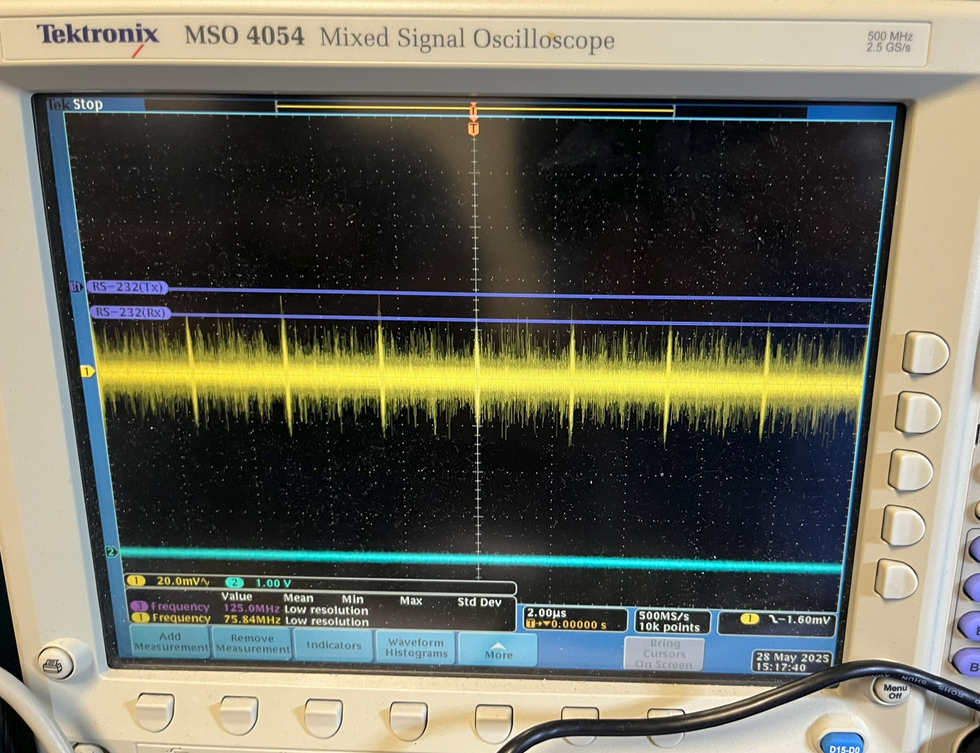
\includegraphics[scale=0.75]{images/dcdc_switching.png}
                    \caption{DC-DC converter switching waveform}
                \label{dcdc_switching}
            \end{figure}
        \item \textbf{Front Panel LEDs} Observe that the LED labeled WIB\_0 is illuminated. \textcolor{blue}{\textbf{Acceptance criteria: PASS/FAIL}}.
        \item \textbf{Repeat} with each of the other 5 DC-DC converters. So, for instance, the second converter will be set to 8b 0000 0010 on SWT1, and RIPPLE\_1 will be measured, and the front panel LED labeled WIB\_1 will be observed. Acceptance criteria are the same in all cases.
        \item \textbf{IMPORTANT:} All DIP switches must be left in the OFF position before moving on to the SoM tests.
        \item Power off PTC, disconnect all cables.
        \item Remove PTC from the QC board test stand by inserting Allen wrenches into the holes on the support structure on each side, and using the wrenches as levers to lift PTC up and away from the QC test stand. 
        \item Re-install the clear plastic plate on the QC test stand for the remaining tests.
    \end{enumerate} 

\subsubsection{SoM Tests}
\label{section:som_tests}

    \begin{enumerate}
        \item \textbf{Install Test} 
            \begin{enumerate}
                \item Scan the Enclustra module QR code, and enter this to be tracked in the database. 
                \item Ensure that the Enclustra SoM can be inserted into connector with no excessive force. Do not force the connectors to mate to avoid bending connector pins or damaging the SoM. \textcolor{blue}{\textbf{Acceptance criteria: PASS/FAIL, with the serial number noted in HWDB}}.
                \item \textbf{IMPORTANT: observe the polarity of the Enclustra SoM when inserting! There are two sets of unequally spaced holes on each side of the SoM that must line up with the corresponding holes in the PTC.} 
                \item After the SoM is installed, re-insert the DUT into the QC test stand.
            \end{enumerate}
        \item \textbf{Boot Test}
            \begin{enumerate}
                \item Turn on the 48V power supply. Initially, PTC will consume about 100-200mA. After a few seconds, the amber LED on the Enclustra board will start blinking at a few Hz and remain blinking. If the amber LED is solid on, or fails to come on, contact a UPenn electronics engineer for assistance.
                \item Ensure that the front panel LED labeled 12V\_LOCAL is illuminated. \textcolor{blue}{\textbf{Acceptance criteria: PASS/FAIL}}.
                \item Ensure front panel PG LED is illuminated. \textcolor{blue}{\textbf{Acceptance criteria: PASS/FAIL}}.
                \item Ensure front panel FPGA DONE LED is illuminated. \textcolor{blue}{\textbf{Acceptance criteria: PASS/FAIL}}.
                \item Ensure the serial port can be connected to. It will come up as /dev/ttyUSB[x], where x is typically 0 or 1 (since there are two serial interfaces in the system -- PTC and QC board). The settings should be: 115,200 baud, 8 bits, no parity bits, 1 stop bit, no hardware flow control. The login name is root. \textcolor{blue}{\textbf{Acceptance criteria: PASS/FAIL}}.
            \end{enumerate}
        \item \textbf{Repeat Boot} Issue the command \texttt{init 0 } at the DUT serial port and wait for the prompt to return a message that it has stopped all services. Turn power off for 60 seconds, and then back on again. Repeat the bootup procedure 5 times. \textcolor{blue}{\textbf{Acceptance criteria: PASS/FAIL}}.
    \end{enumerate}    
    
%%%%%%%%%%%%%%%%%%%%%%%%%%%%%%%%%%%%%%%%%%%%%%%%%%%%%%%
\newpage
\subsection{Semi-automated QC Tests}
\label{section:auto_tests}

\subsubsection{DC-DC Converter Load Test}
\label{section:load_tests}
    \begin{enumerate}
        \item \textbf{Setup} Boot up the DUT again while it is plugged into the powered-on QC board. Now commands will be issued on the DUT and QC board to exercise different loads.
        \item \textbf{Turn on PTC} While ssh'd into the DUT, type \texttt{python3 power\_on\_wib.py 0 on} for the first DC-DC converter.
        \item \textbf{Enable PWM driver} While ssh'd into the QC board, type \texttt{poke 0x80020038 0x316} followed by the value \texttt{0x216}. This sets the PWM driver to 2MHz and 25\% duty cycle.
        \item \textbf{Measure current draw} The DUT should be drawing approximately 1.5A. Confirm on the 48V power supply that the current consumption has increased by 500mA (Note that the current consumption of 2A at 12V is equivalent to 500mA at 48V. There is some inefficiency in the converter -- the load side current will be measured more accurately with I2C sensors in the next section.) \textcolor{blue}{\textbf{Acceptance criteria: $1.5A\pm100mA$}}.
        \item \textbf{Repeat with other load values} The values of \texttt{0x226, 0x236, 0x23e} will test 50\%, 75\%, and approximately 100\% load on the converter. Confirm the coresponding current draws are 3A, 4.5A, and 6A. \textcolor{blue}{\textbf{Acceptance criteria: $3A\pm100mA$, $4.5A\pm100mA$, $6A\pm100mA$}}.
        \item \textbf{Measure voltage ripple} At the highest load, measure the test point RIPPLE\_0 with the scope set on 200mV scale, 200ns period, and AC coupling, and note the AC ripple. \textcolor{blue}{\textbf{Acceptance criteria: $\pm200mV$}}. An example is shown in Figure~\ref{dcdc_ripple}.
            \begin{figure}[h!]
                \centering             
                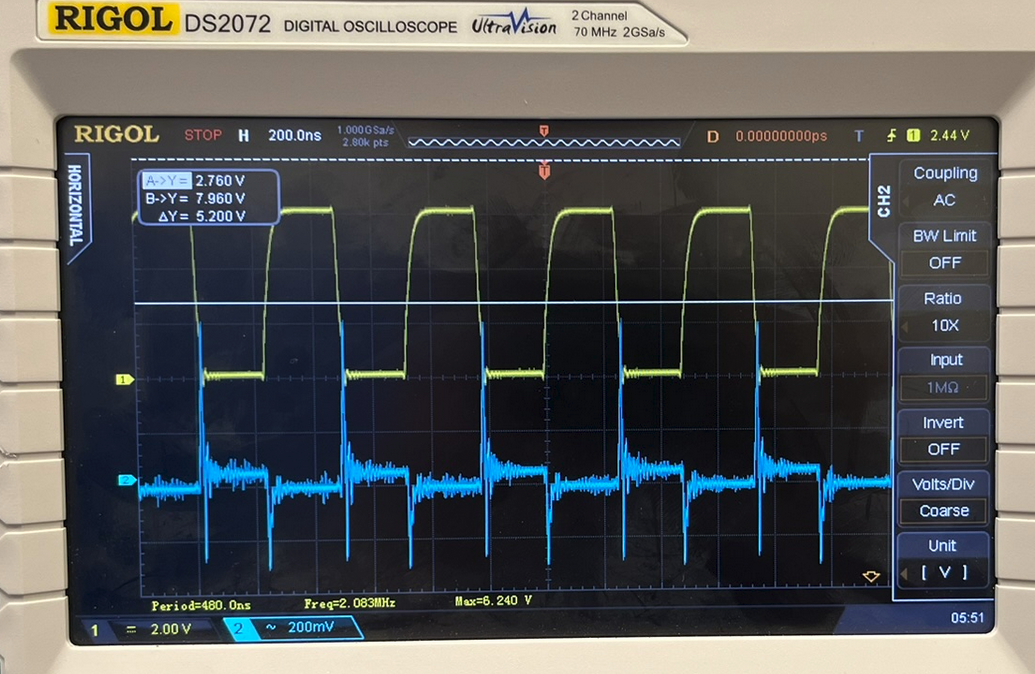
\includegraphics[scale=0.75]{images/dcdc_ripple.png}
                    \caption{Example of ripple measurement (CH2, blue)}
                \label{dcdc_ripple}
            \end{figure}
        \item \textbf{Repeat with other converters} The addresses of \texttt{0x8002003c, 0x80020040, 0x80020044, 0x80020048, 0x8002004c} correspond to converters 1 through 5. Repeat the test for all converters. Acceptance criteria are same as above.
    \end{enumerate}

\subsubsection{I2C Sensor Tests}
\label{section:i2c_tests}

    \begin{enumerate}
        \item \textbf{Setup} The test script will simultaneously test all sensors in the list below, as well at the EtherCAT link in the QC tests below.
            \begin{enumerate}
                \item On the DUT, turn all DC-DC converters on with \texttt{python3 power\_on\_wib.py [x] on} where the command is repeated 6 times with [x] being 0--5.
                \item Then, on the DUT, run \texttt{python3 ecat\_test\_1b.py [filename].txt} where filename is the logfile; choose any name (for example, the serial number of the DUT).
                \item A sample output is shown in Figure~\ref{i2c_output}. The full set of values to be written into the HWDB will be parsed by a Python scope (to be written) and assigned PASS/FAIL values based on the acceptance criteria.
            \end{enumerate}
            \begin{figure}[h!]
                \centering             
                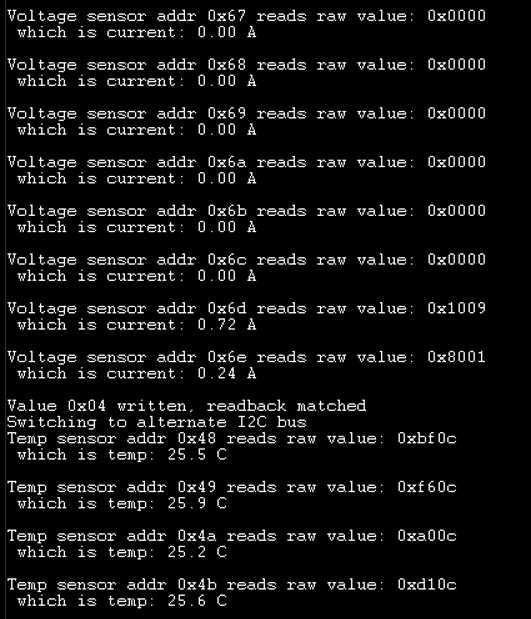
\includegraphics[scale=1.25]{images/i2c_output.png}
                    \caption{A sample selection of I2C output. Note: no load applied.}
                \label{i2c_output}
            \end{figure}
        \item \textbf{Main DC-DC Converter Sensors}
            \begin{enumerate}
                \item Voltage. Each 12V output to WIB is read from the sensor. \textcolor{blue}{\textbf{Acceptance criteria: 12.00 -- 12.35V}}.
                \item Current. Measured at 25\% load. The purpose of this test is to ensure the current measurement resistor is installed and the correct value, so a comprehensive tests at different loads does not need to be repeated. \textcolor{blue}{\textbf{Acceptance criteria: $1.5A\pm100mA$}}.
            \end{enumerate}
        \item \textbf{SoM Sensor}
            \begin{enumerate}
                \item Voltage. \textcolor{blue}{\textbf{Acceptance criteria: 12.00 -- 12.35V}}.
                \item Current. \textcolor{blue}{\textbf{Acceptance criteria: $\leq2A$}}.
            \end{enumerate}
        \item \textbf{Auxiliary Sensors}
            \begin{enumerate}
                \item 2.5V Local Voltage. \textcolor{blue}{\textbf{Acceptance criteria: 2.4 -- 2.6V}}.
                \item 2.5V Local Current. \textcolor{blue}{\textbf{Acceptance criteria: $\leq2A$}}.
                \item 3.3V Local Voltage. \textcolor{blue}{\textbf{Acceptance criteria: 3.2 -- 3.4V}}.
                \item 3.3V Local Current. \textcolor{blue}{\textbf{Acceptance criteria: $\leq2A$}}.
            \end{enumerate}
        \item \textbf{Temperature Sensors}. All 8 temperature sensors should read close to ambient temperature. Since there are variations in air flow, local board temperature based on how long a DC-DC converter was recently switched on or off, the acceptance criteria is not strict. The purpose of the test is to ensure that the temperature sensors are installed. \textcolor{blue}{\textbf{Acceptance criteria: Ambient temperature $\pm5C$}}.
        \item \textbf{Sensor Extended Functionality}
            \begin{enumerate}
                \item ALARM. From the QC\_DEV branch of the github repository, run the \\ 
                \verb|qc_firmware\scripts\test_scripts\alert_assert.py| script. This will go through each sensor, program a threshold such that the ALERT pin is asserted, and readback the ALERT register over I2C. \textcolor{blue}{\textbf{Acceptance criteria: PASS/FAIL}}.
                \item Front panel OVER TEMP LED. For any of the above ALARM line asserts, the OVER TEMP LED should illuminate in RED on the front panel. \textcolor{blue}{\textbf{Acceptance criteria: PASS/FAIL}}.
            \end{enumerate}
    \end{enumerate}   

\subsubsection{Addressing}
\label{section:addr_tests}

    \begin{enumerate}
        \item \textbf{Crate Address DIP Switch}. 
            \begin{enumerate}
                \item Temporarily remove the clear plastic plate on the QC test stand.
                \item For each of the 8 DIP switches, switch to ON position with tweezers or a small flathead screwdriver.
                \item Ensure the corresponding crate address ID is illuminated. \textcolor{blue}{\textbf{Acceptance criteria: PASS/FAIL}}.
                \item Re-install the clear plastic plate on the test stand.
            \end{enumerate}
        \item \textbf{EEPROM R/W Test}. From the QC\_DEV branch of the github repository, run the \\ 
        \verb|qc_firmware\scripts\test_scripts\eeprom.py| script. This will read the globally unique serial ID from the EEROM. \textcolor{blue}{\textbf{Acceptance criteria: PASS/FAIL, with serial number noted in HWDB}}.
    \end{enumerate}

\subsubsection{Microcontroller Tests}
\label{section:mcu_tests}

    \begin{enumerate}
        \item \textbf{Setup} The complete setup instructions are shown on the PTC github page README, and are repeated here for clarity:
            \begin{enumerate}
                \item The EtherCAT microcontroller project is based on the Infineon reference design. Ensure that the same version of tools are installed. Beckhoff TwinCAT3 is needed to initiate a connection to PTC. Infineon DAVE v4.1.4 or higher and the Beckhoff SSC tool v5.12 are used for creating the initial project, but is only needed for development.
                \item The first time the link is set up, or if any configuration changes, copy the XMC\_ESC.xml file (the "ESI file") to \\
                \verb|C:\TwinCAT\3.1\Config\Io\EtherCAT| on the host PC.
                \item Connect a 100Base-FX SFP to SFP1, with an LC-to-SC fiber connection. For bench testing, this can be connected to a optical-to-fiber converter (like the tp-link MC100CM). 
                \item From the main branch in github, open up the TwinCAT project in the \texttt{ethercat/} directory.
                \item Now program the microcontroller.
            \end{enumerate}
        \item \textbf{Program MCU}
            \begin{enumerate}
                \item Programming over JTAG cable. After connecting the Infineon XMC Link cable to J14, click on the "Debug" button (looks like a bug) in the DAVE project opened in the previous step. This will compile and load the project. \textcolor{blue}{\textbf{Acceptance criteria: PASS/FAIL}}.
                \item In-situ programming using FPGA. After obtaining a shell, run the command \newline \verb|openocd -f ptc-flash.cfg -c "set FIRMWARE { /home/root/xmc4300_firm.elf }|.
                \textcolor{blue}{\textbf{Acceptance criteria: PASS/FAIL}}.
            \end{enumerate}
        \item \textbf{Test EtherCAT Link}
        \begin{enumerate}
            \item Double click on "Device 1 (EtherCAT)" and click on the "Adapter" panel. Ensure that the correct PTC Ethernet interface is selected.
            \item Right click on Device 1, and click "Scan". A message saying "Configuration matched" should appear.
            \item Now click on the "Online" tab. PTC should appear as a "Box" and be labeled "XMC\_ESC".
            \item In the top menu bar, click on the "Toggle Free-Run State" icon (a red circular arrow).
            \item Front panel LINK LED. \textcolor{blue}{\textbf{Acceptance criteria: PASS/FAIL}}.
            \item TwinCAT link test. Now the PTC can be changed to "Op" mode in the Online panel. There will be constant frame counters in this panel, and no lost frames. This means PTC is maintaining an EtherCAT link. The PTC Debug LEDs will show: ERR=GREEN, LINKB=GREEN, PHY\_KED2=BLINK GREEN. \textcolor{blue}{\textbf{Acceptance criteria: PASS/FAIL}}.
            \item Front panel ECAT RUN LED. \textcolor{blue}{\textbf{Acceptance criteria: PASS/FAIL}}.
        \end{enumerate}
    \end{enumerate}    

\subsubsection{Timing}
\label{section:timing_tests}

Note that the timing system was set up in a previous step, and should be in a state where it is transmitting valid information.

    \begin{enumerate}
        \item \textbf{RX Test}. Run the following sequence of commands:
        \begin{enumerate}
            \item Timing lock
\begin{verbatim}
root@ptc:~# python3 setup_timing.py
root@ptc:~# poke 0x80020004 0x00010400
root@ptc:~# peek 0x80020104
0x00073f00 # timing endpoint reset
root@ptc:~# poke 0x80020004 0x00010000
root@ptc:~# peek 0x80020104
0x18073f00 # endpoint out of reset, and showing 0x8 status (good)
\end{verbatim}
        \textcolor{blue}{\textbf{Acceptance criteria: PASS/FAIL}}.
            \item Front panel LINK LED. \textcolor{blue}{\textbf{Acceptance criteria: PASS/FAIL}}.
            \item Front panel RX LED. \textcolor{blue}{\textbf{Acceptance criteria: PASS/FAIL}}.
        \end{enumerate}
        \item \textbf{TX Test}
            \begin{enumerate}
                \item To measure round trip time, run the following sequence of commands:
\begin{verbatim}
dtsbutler -c local.xml mst MST_FMC align measure-delay 0 
    # should get ~100 clock ticks
dtsbutler -c local.xml mst MST_FMC align toggle-tx 0 --on|off 
    # should turn LED on
\end{verbatim}
                The RTT in milliseconds should be displayed. The RTT will vary based on testing conditions, so the purpose of the test is to ensure that the priority encoder and clock multiplexer are installed correctly, and that that the timing stream is routed back through the front panel. \textcolor{blue}{\textbf{Acceptance criteria: PASS/FAIL}}.
                \item Front panel TX LED. The LED will temporarily illuminate when the RTT test is conducted. \textcolor{blue}{\textbf{Acceptance criteria: PASS/FAIL}}.
            \end{enumerate}
    \end{enumerate}    

\subsubsection{Ethernet Tests}
\label{section:eth_tests}

    \begin{enumerate}
        \item \textbf{Ping Test}
            \begin{enumerate}
                \item Front panel LINK LED. \textcolor{blue}{\textbf{Acceptance criteria: PASS/FAIL}}.
                \item Ping. The DUT should come up as 192.168.200.10 on the network. Issue the \texttt{ping} commands from the Linux test machine and ensure the DUT responds. \textcolor{blue}{\textbf{Acceptance criteria: PASS/FAIL}}.
            \end{enumerate}
        \item \textbf{Throughput Test}. You can ssh into the PTC as user root. 
        Use the \texttt{dd} command to transfer the 1GB file called \texttt{thru\_test.bin} to \verb|/dev/null|. \textcolor{blue}{\textbf{Acceptance criteria: $>12.5MB/s$}}.
        \item \textbf{Front Panel AUX LED}. Illuminate the LED by writing the register address \texttt{\textcolor{red}{TBD}}. Note: this is a spare LED that may have a future functionality related to the GbE interface. For now, it is toggled with a register bit. \textcolor{blue}{\textbf{Acceptance criteria: PASS/FAIL}}.
    \end{enumerate}

%%%%%%%%%%%%%%%%%%%%%%%%%%%%%%%%%%%%%%%%%%%%%%%%%%%%%%%
\newpage
\subsection{Mechanical Installations}
\label{section:mechanical}

    \begin{enumerate}
        \item \textbf{Heatsink Install}
            \begin{enumerate}
                \item Clean the top of the LTM-8064 DC-DC converters with an alcohol swab.
                \item The thermal interface material (TIM) has double sided adhesive. Remove one side of the adhesive, and apply to the top of each LTM-8064.
                \item Remove the other side of the adhesive on the TIM and apply the heatsink with even pressure. An example of installed heatsinks is shown in Figure ~\ref{heatsink_pcb}. 
                \begin{figure}[h!]
                \centering             
                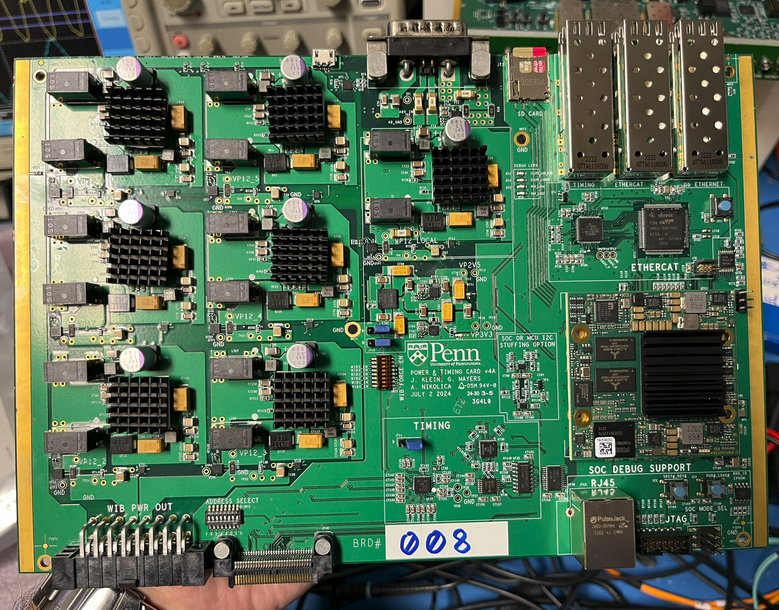
\includegraphics[scale=0.9]{images/heatsink_pcb.png}
                    \caption{PTC with installed heatsinks}
                \label{heatsink_pcb}
                \end{figure}
            \end{enumerate}
        \item \textbf{Front Panel Install}
            \begin{enumerate}
                \item Insert light pipes into each LED hole and secure with rubber grommet. 
                \item Attach the front panel to the DUT at the 2 L-bracket locations. is shown in Figure ~\ref{panel_pcb}. 
                \begin{figure}[h!]
                \centering             
                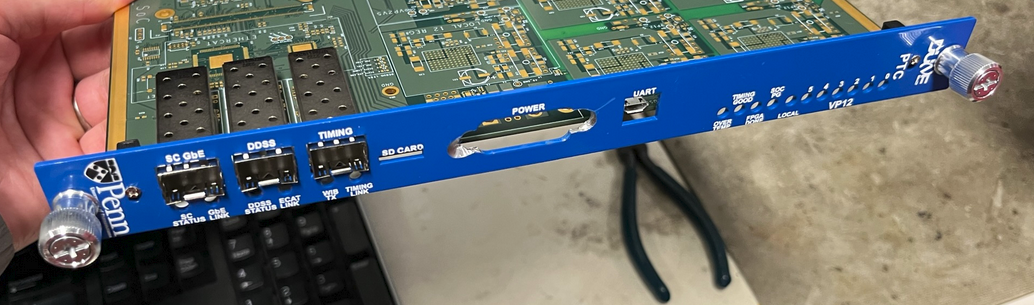
\includegraphics[scale=0.8]{images/panel_pcb.png}
                    \caption{PTC with installed front panel. Note: light pipes not shown in this picture.}
                \label{panel_pcb}
                \end{figure}
            \end{enumerate}
        \item \textbf{Packing} The PTC is now ready to be packed in an ESD bag and placed in a secure location for shipment. Ensure that the overall test result for the DUT is entered in the HWDB. \textcolor{blue}{\textbf{Acceptance criteria: PASS/FAIL}}. 
    \end{enumerate}

%%%%%%%%%%%%%%%%%%%%%%%%%%%%%%%%%%%%%%%%%%%%%%%%%%%%%%%
\newpage
\subsubsection{QC Test Stand Tear-down}
\label{section:qc_teardown}

After testing is finished for a shift, uninstall any DUT still plugged in. On the QC board, issue the command \texttt{init 0} and wait for the power-down message (a few seconds). Then power off the 24V to the QC board. Finally, power off the 12V to the QC heatsink fans.
    
%%%%%%%%%%%%%%%%%%%%%%%%%%%%%%%%%%%%%%%%%%%%%%%%%%%%%%%
\newpage
\subsection{WEIC Tests of a Sample of PTCs}
\label{section:crate_tests}

A subsample of fully tested and assembled PTCs (including heatsinks and front panels) will be sent to BNL for insertion into a WEIC, as in Figure~\ref{weic}. For this test, the sample PTCs will be instrumented with temperature sensors on each of the main 12V DC-DC converters before insertion into the crate. Then 6 WIBs will be powered on via the PTC, and all FEMBs will be turned on and configured for nominal operating conditions. The procedures for this are defined in the WIB QC procedure.
    \begin{figure}[h!]
        \centering             
        \includegraphics[scale=1.25]{images/weic.png}
            \caption{PTC inserted into WEIC}
        \label{weic}
    \end{figure}

Temperature as measured on top of heatsinks \textcolor{blue}{\textbf{Acceptance criteria: $<60C$}} for all heatsinks.

%%%%%%%%%%%%%%%%%%%%%%%%%%%%%%%%%%%%%%%%%%%%%%%%%%%%%%%%%%%%%%%%%%
\newpage
\section{End of Shift Checklist}
\label{app:results}


\textbf{Date:}\\
\textbf{Time:}\\
\textbf{Tester's Name:} \\

\vskip 2 cm 



\begin{table}[h!]
\centering
\renewcommand{\arraystretch}{2.0}
\begin{tabularx}{\textwidth}{|l|c|X|}
\hline
\textbf{Tested PTC SN} & \textbf{Result (PASS/FAIL/Other)} & \textbf{Comments} \\
\hline
 &  &  \\ \hline
 &  &  \\ \hline
 &  &  \\ \hline
 &  &  \\ \hline
 &  &  \\ \hline
\end{tabularx}
%\caption{CE Box Preparation Checklist.}
\label{tab:results}
\end{table}

\vskip 2 cm
\textbf{Notes:}\\
 
   
\end{document}
%%%%%%%%%%%%%%%%%%%%%%%%%%%%%%%%%%%%%%%%%%%%%%%%%%%%%%%